\chapter[Practical Hybrid Quantum-Classical Computing]{Practical Hybrid Quantum-Classical\\Computing} \label{chap:practical-hybrid-quantum-classical-computing}
This chapter is focused on the practical execution of \glspl{hqca} using the Quantum Inspire quantum computing platform and SURF's \gls{hpc} center.
First, an overview of the quantum computing platform Quantum Inspire is given.
%Then, \glspl{hqca} discussed in \Cref{chap:hybrid-quantum-classical-algorithms} are implemented and used for benchmarking and identifying the bottlenecks of the current infrastructure.
% TODO: describe sections

\section{Quantum Inspire}
Quantum Inspire is a full-stack quantum computing platform that QuTech launched last year to make quantum systems available to the general public for exploratory research~\cite{last2020quantum}.
Users can run quantum circuits on different back-ends through the Quantum Inspire web editor or by using the Python \gls{sdk}.
The \gls{cqasm}~\cite{khammassi2018cqasm} is used for describing quantum circuits, but the popular quantum computing frameworks ProjectQ~\cite{steiger2018projectq} and Qiskit~\cite{qiskit} are also supported by the Python \gls{sdk}.

\subsection{Back-Ends}
Quantum Inspire supports the execution of quantum circuits on real quantum chips and through quantum simulation.
An overview of the Quantum Inspire workflow and available device back-ends is shown in \Cref{fig:qi-workflow}.
% queue, fifo
% absence of large quantum computers, quantum computer simulation is critical for developing and testing quantum algorithms
\begin{figure}[ht]
    \centering
    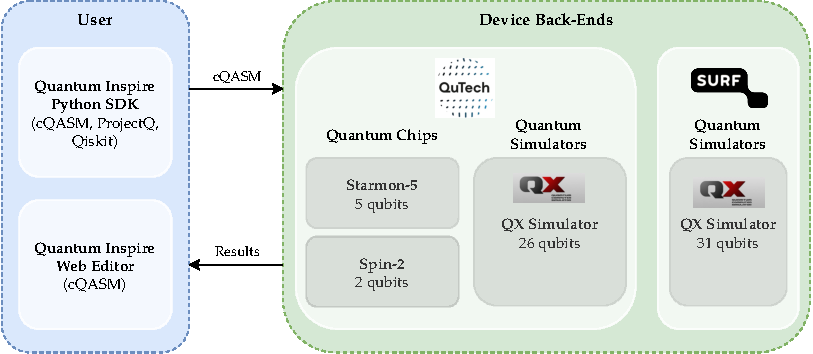
\includegraphics[width=1\linewidth]{figures/qi-workflow.pdf}
    \caption[Overview of the Quantum Inspire workflow.]{
        Overview of the Quantum Inspire workflow.
        Users can submit quantum circuits written in \gls{cqasm} using the web editor or Python \gls{sdk}.
        After the program has been run, the results are returned to the user.
        The quantum circuit can be executed on one of the quantum chips or simulated using one of the QX simulator back-ends.
        QuTech's simulator back-end supports simulations up to 26 qubits, while SURF's simulator back-end supports simulations up to 31 qubits.
    }
    \label{fig:qi-workflow}
\end{figure}

\subsection{cQASM}

\section{Implementation}